\subsection{Cremmer-Gervais $i \mapsto i-1$}
The initial quiver for $\gc_g^{\dagger}(\bg,\GL_4)$ is illustrated in Figure~\ref{f:ex_n=4cg}.

\begin{figure}[htb]
\begin{center}
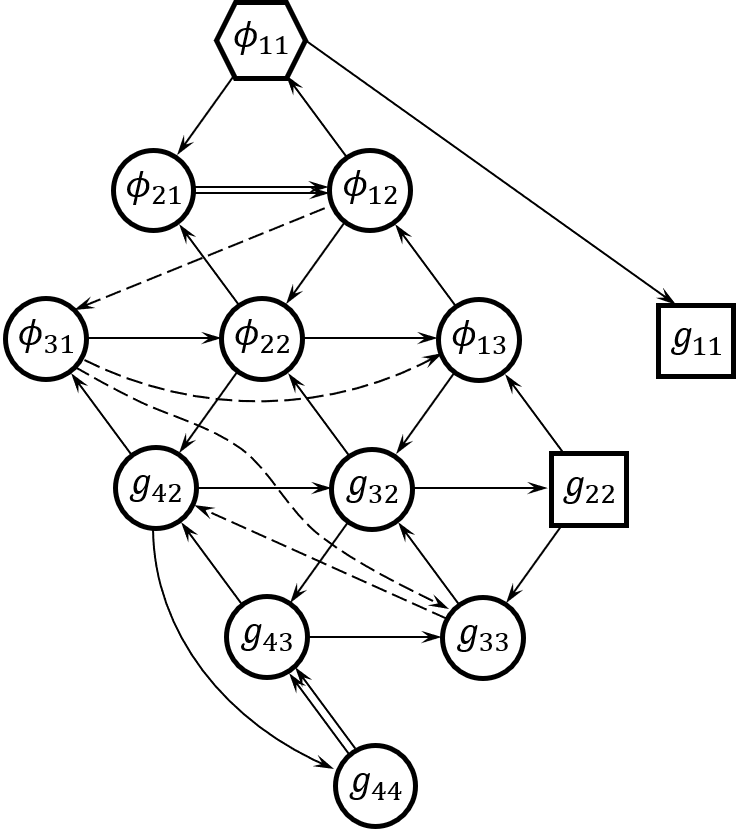
\includegraphics[scale=0.65]{g_convention/g_n=4_cg_i-i-1.png}
\end{center}
\caption{The initial quiver for $\gc^{\dagger}_g(\bg,\GL_4)$ for $\Gamma_1 = \{2,3\}$, $\Gamma_2 = \{1,2\}$, $\gamma:i \mapsto i-1$.}
\label{f:ex_n=4cg}
\end{figure}

\paragraph{The initial variables.} Let us set
\begin{align}
    &\ell_1(U) := \det U^{[3,4]}_{[3,4]}u_{44} +\det U^{\{2,4\}}_{[3,4]} u_{34}+ \det U_{[3,4]}^{\{1,4\}} u_{24};\\
    &\ell_2(U) := \det U^{[3,4]}_{\{2,4\}}u_{44} +\det U^{\{2,4\}}_{\{2,4\}} u_{34}+ \det U_{\{2,4\}}^{\{1,4\}} u_{24};\\
    &\ell_3(U) := \det U^{[3,4]}_{[2,3]}u_{44} +\det U^{\{2,4\}}_{[2,3]} u_{34}+ \det U_{[2,3]}^{\{1,4\}} u_{24}.
\end{align}
The $g$-variables are given by the following formulas:
\begin{align}
    &g_{42}(U) = u_{42}\cdot \ell_1(U) + u_{41}\ell_2(U), \ \ g_{43}(U) = u_{43}u_{44} + u_{42}u_{34} + u_{41}u_{24}, \ \ g_{44}(U) = u_{44}; \\
    &g_{32}(U) = \det U_{[3,4]}^{[2,3]}\ell_1(U) + \det U_{[3,4]}^{\{1,3\}}\ell_2(U) + \det U_{[3,4]}^{[1,2]}\ell_3(U), \ \ g_{33}(U) = \ell_1(U);\\
    &g_{22}(U) = \det U_{[2,4]}^{[2,4]}\ell_1(U) + \det U^{\{1\}\cup[3,4]}_{[2,4]}\ell_2(U) + \det U_{[2,4]}^{[1,2]\cup\{4\}}\ell_3(U).
\end{align}

\paragraph{Birational quasi-isomorphisms.} There is a birational quasi-isomorphism
\begin{equation}
    \mathcal{Q}^{\op}: (\GL_4,\gc_g^{\dagger}(\bg_{\std})) \dashrightarrow (\GL_4,\gc_g^{\dagger}(\bg)), \ \ \mathcal{Q}^{\op}(U):=\rho^{\op}(U)U (\rho^{\op}(U))^{-1}
\end{equation}
where the rational map $\rho^{\op}:\GL_n \dashrightarrow \GL_n$ is given by
\begin{equation}
    \rho^{\op}(U) = \left(I+\frac{u_{34}}{u_{44}}e_{12}\right)\cdot \left(I + \frac{\det U_{\{2,4\}}^{[3,4]}}{\det U^{[3,4]}_{[3,4]}}e_{12} + \frac{u_{24}}{u_{44}}e_{13} + \frac{u_{34}}{u_{44}}e_{23}\right).
\end{equation}
The marked variables for $\mathcal{Q}^{\op}$ are $g_{33}$ and $g_{44}$. Define the BD triples $\tilde{\bg}:=(\{2\},\{1\},2\mapsto 1)$ and $\hat{\bg}:=(\{3\},\{2\},3\mapsto 2)$. There is a pair of complementary birational quasi-isomorphisms 
\begin{equation}\mathcal{G}:(\GL_4,\gc_g^{\dagger}(\tilde{\bg})\dashrightarrow (\GL_4,\gc_g^{\dagger}(\bg)), \ \ \mathcal{G}^\prime:(\GL_4,\gc_g^{\dagger}(\hat{\bg})) \dashrightarrow (\GL_4,\gc_g^{\dagger}(\bg)).
\end{equation}
They are given by
\begin{align}
    \mathcal{G}^{\op}(U) &= G^{\op}(U)\cdot U \cdot G^{\op}(U)^{-1}, \ \ G^{\op}(U) := \left(I+\frac{u_{34}}{u_{44}}e_{12}\right)\cdot \left(I+\frac{u_{24}}{u_{44}}e_{13} + \frac{u_{34}}{u_{44}}e_{23}\right);
    \end{align}
    \begin{align}
   (\mathcal{G}^\op)^\prime(U) &= G^\prime(U)\cdot U \cdot G^{\prime}(U)^{-1}, \ \ G^{\prime}(U) := (I+\alpha_1(U) e_{12} + \alpha_2(U) e_{13}),\\
    \alpha_1(U) &= \frac{\det U^{[3,4]}_{\{2,4\}}u_{44} + \det U_{\{2,4\}}^{\{2,4\}}u_{34}}{\det U^{[3,4]}_{[3,4]}u_{44} + \det U_{[3,4]}^{\{2,4\}}u_{34}}, \ \ \alpha_2(U) = -\frac{\det U^{[3,4]}_{[2,3]}u_{44} + \det U_{[2,3]}^{\{2,4\}}u_{34}}{\det U^{[3,4]}_{[3,4]}u_{44} + \det U_{[3,4]}^{\{2,4\}}u_{34}}.
\end{align}
The marked variable for $\mathcal{G}$ is $g_{44}$, and the marked variable for $\mathcal{G}^\prime$ is $g_{33}$.

%The full description of $\gc_g^{\dagger}(\tilde{\bg})$ and $\gc_g^{\dagger}(\hat{\bg})$ (along with more examples) is available on the author's github repository (see the previous section).
